\def\year{2021}\relax
% File: formatting-instruction.tex
\documentclass[letterpaper]{article}
% DO NOT CHANGE THIS
\usepackage{aaai21} % DO NOT CHANGE THIS
\usepackage{times} % DO NOT CHANGE THIS
\usepackage{helvet} % DO NOT CHANGE THIS
\usepackage{courier} % DO NOT CHANGE THIS
\usepackage[hyphens]{url} % DO NOT CHANGE THIS
\usepackage{graphicx} % DO NOT CHANGE THIS
\urlstyle{rm} % DO NOT CHANGE THIS
\def\UrlFont{\rm} % DO NOT CHANGE THIS
\usepackage{graphicx}  % DO NOT CHANGE THIS
\usepackage{natbib}
% DO NOT CHANGE THIS OR ADD OPTIONS
\usepackage{caption}
% DO NOT CHANGE THIS OR ADD OPTIONS
\usepackage{algorithm}
\usepackage{algpseudocode}
\usepackage{float}
\usepackage{subfig}
\usepackage{xcolor}
\usepackage{amssymb}
\usepackage{mathtools}
\usepackage{amsthm}
\frenchspacing % DO NOT CHANGE THIS
\setlength{\pdfpagewidth}{8.5in} % DO NOT CHANGE THIS
\setlength{\pdfpageheight}{11in} % DO NOT CHANGE THIS

\theoremstyle{definition}
\newtheorem{definition}{Definition}
%\newtheorem{definition}{Definition}[section]

\frenchspacing  % DO NOT CHANGE THIS
\setlength{\pdfpagewidth}{8.5in}  % DO NOT CHANGE THIS
\setlength{\pdfpageheight}{11in}  % DO NOT CHANGE THIS

\newtheorem{example}{Example}

\newcommand{\commentout}[1]{}
\newcommand{\eliran}[1]{\textbf{[\color{red}ELIRAN:#1]}}
\newcommand{\ronen}[1]{\textbf{[\color{blue}RONEN:#1]}}
\newcommand{\guy}[1]{\textbf{[\color{orange}GUY:#1]}}
%\newcommand{\begin{example}}[1]{\textbf{[\color{purple}RunningExample:#1]}}

\newcommand{\cbp}[0]{Collaborative Box-Pushing}
\newcommand{\cdt}[0]{Collaborative Dec-Tiger}
\newcommand{\drs}[0]{Decentralized Rock-Sampling}
\newcommand{\crs}[0]{Cooperative Rock-Sampling}
\newcommand{\macor}[0]{Multi-Agent Corridor}

\newcommand{\cact}[1]{{\em CActions$_#1$}}
\newcommand{\mcact}[1]{{\mathit{CActions}_#1}}
\newcommand{\pcact}[1]{{\mathit{PCA}_#1}}
\newcommand{\eff}{\mathit{eff}}
\newcommand{\rel}{\mathit{rel}}
\newcommand{\Tau}{\mathrm{T}}
\newcommand{\infl}{\mathit{inf}}

%\nocopyright
%PDF Info Is REQUIRED.
% For /Author, add all authors within the parentheses, separated by commas. No accents or commands.
% For /Title, add Title in Mixed Case. No accents or commands. Retain the parentheses.
 \pdfinfo{
/Title (A Factored Approach To Solving Dec-POMDPs)
/Author (Eliran Abdoo, Ronen I. Brafman, Guy Shani)
} %Leave this	
% /Title ()
% Put your actual complete title (no codes, scripts, shortcuts, or LaTeX commands) within the parentheses in mixed case
% Leave the space between \Title and the beginning parenthesis alone
% /Author ()
% Put your actual complete list of authors (no codes, scripts, shortcuts, or LaTeX commands) within the parentheses in mixed case. 
% Each author should be only by a comma. If the name contains accents, remove them. If there are any LaTeX commands, 
% remove them. 

% DISALLOWED PACKAGES
% \usepackage{authblk} -- This package is specifically forbidden
% \usepackage{balance} -- This package is specifically forbidden
% \usepackage{caption} -- This package is specifically forbidden
% \usepackage{color (if used in text)
% \usepackage{CJK} -- This package is specifically forbidden
% \usepackage{float} -- This package is specifically forbidden
% \usepackage{flushend} -- This package is specifically forbidden
% \usepackage{fontenc} -- This package is specifically forbidden
% \usepackage{fullpage} -- This package is specifically forbidden
% \usepackage{geometry} -- This package is specifically forbidden
% \usepackage{grffile} -- This package is specifically forbidden
% \usepackage{hyperref} -- This package is specifically forbidden
% \usepackage{navigator} -- This package is specifically forbidden
% (or any other package that embeds links such as navigator or hyperref)
% \indentfirst} -- This package is specifically forbidden
% \layout} -- This package is specifically forbidden
% \multicol} -- This package is specifically forbidden
% \nameref} -- This package is specifically forbidden
% \natbib} -- This package is specifically forbidden -- use the following workaround:
% \usepackage{savetrees} -- This package is specifically forbidden
% \usepackage{setspace} -- This package is specifically forbidden
% \usepackage{stfloats} -- This package is specifically forbidden
% \usepackage{tabu} -- This package is specifically forbidden
% \usepackage{titlesec} -- This package is specifically forbidden
% \usepackage{tocbibind} -- This package is specifically forbidden
% \usepackage{ulem} -- This package is specifically forbidden
% \usepackage{wrapfig} -- This package is specifically forbidden
% DISALLOWED COMMANDS
% \nocopyright -- Your paper will not be published if you use this command
% \addtolength -- This command may not be used
% \balance -- This command may not be used
% \baselinestretch -- Your paper will not be published if you use this command
% \clearpage -- No page breaks of any kind may be used for the final version of your paper
% \columnsep -- This command may not be used
% \newpage -- No page breaks of any kind may be used for the final version of your paper
% \pagebreak -- No page breaks of any kind may be used for the final version of your paperr
% \pagestyle -- This command may not be used
% \tiny -- This is not an acceptable font size.
% \vspace{- -- No negative value may be used in proximity of a caption, figure, table, section, subsection, subsubsection, or reference
% \vskip{- -- No negative value may be used to alter spacing above or below a caption, figure, table, section, subsection, subsubsection, or reference

\setcounter{secnumdepth}{2} %May be changed to 1 or 2 if section numbers are desired.

% The file aaai20.sty is the style file for AAAI Press 
% proceedings, working notes, and technical reports.
%
\setlength\titlebox{2.5in} % If your paper contains an overfull \vbox too high warning at the beginning of the document, use this
% command to correct it. You may not alter the value below 2.5 in
\title{A Factored Approach To Solving Dec-POMDPs }
%Your title must be in mixed case, not sentence case. 
% That means all verbs (including short verbs like be, is, using,and go), 
% nouns, adverbs, adjectives should be capitalized, including both words in hyphenated terms, while
% articles, conjunctions, and prepositions are lower case unless they
% directly follow a colon or long dash
\author{Submission 74}
% \author{Eliran Abdoo, Ronen I Brafman, Guy Shani\\
% Ben-Gurion University, Israel\\
% eliranb,brafman,shanigu@bgu.ac.il}
\begin{document}

\maketitle

\begin{abstract}
Dec-POMDPs model planning problems under uncertainty and partial observability for a distributed team of cooperating agents planning together but executing their plans in a distributed manner. This problem is
very challenging computationally (NEXP-Time Complete) and consequently, exact methods have difficulty scaling up. In this paper we present a heuristic approach for solving certain instances of Factored Dec-POMDP. Our approach reduces the joint planning problem to multiple single agent POMDP planning problems.
First, we solve a centralized version of the Dec-POMDP, which we call the team problem, where agents have a shared belief state. Then, each agent individually plans to execute its part of the team plan. Finally, the different solutions are aligned to achieve synchronization. Using this approach we are able to scale to larger Dec-POMDP problems, limited mainly by the abilities of the underlying POMDP solver.
\end{abstract}




\section{Introduction}

Decentralized Partially Observable Markov Decision Processes (Dec-POMDPs) are a popular model for planning in stochastic environments under uncertainty with partial observability by a distributed team of agents \cite{DECPOMDPART}. In this model, a team of agents attempts to maximize the team's cumulative reward where each agent has only partial information about the state of the system during execution.  We concentrate on the
well studied case of centralized off-line planning for distributed execution. 
That is, the team can plan together centrally prior to acting, but during execution each agent is aware of its own observations only.  Communication is possible only through explicit communication actions, if these are available. 

%To achieve their common goal agents must coordinate their actions in two ways: First, as in single agent problems, actions must be coordinated sequentially. 
%That is, current actions must help steer the system towards states from which greater reward can be attained. For example, to be rewarded for shipping a product, it must  be assembled first. 
%Second, agents may need to coordinate their simultaneous actions because their effects are dependent, e.g., a heavy box can only be pushed if two agents push it simultaneously. 

%Our focus is on centralized off-line planning for distributed execution. That is, offline, a solver with access to the complete model must generate a policy for each agent. 
A solution to a DecPOMDP is a set of policies -- one for each agent.
%An agent's policy specifies which action it executes as a function of the agent's history of
%actions and observations. Such policies can be represented by a {\em policy graph} where nodes are labeled by actions, and edges are labeled by observations. Online, each agent executes its own policy independently of the other agents.
The challenge is to generate policies that provide sufficient coordination, even though each agent makes different observations at run-time,
and hence, agents' belief states at each point in time are typically different.

Dec-POMDPs are notoriously hard to solve -- they are NEXP-Time hard~\cite{DECPOMDPCOMP}, implying that only the smallest toy problems are optimally solvable.
However, many approximate methods for solving Dec-POMDPs have been proposed, with steady progress. Some of these methods generate solutions with bounds on
their optimality \cite{GMAAICE,MBDP,DICEPS}, and some are heuristic in nature~\cite{JESP}. However, current methods typically do not scale to state spaces with more than a few hundreds of states.


In this paper we describe a heuristic approach for solving Dec-POMDPs that scales to much larger state spaces. The key idea is to solve a Dec-POMDP by
solving multiple POMDPs. First, we solve a {\em team POMDP}
in which every agent's observations are
immediately available to the other agents. Hence, all agents have the same belief state.  The solution of the team
POMDP can be represented by a policy graph --- the {\em team policy graph}. We view this
graph as a skeleton for solution of the true Dec-POMDP. It specifies what each agent needs to provide for the team. 

This team policy graph is not executable by the agents, because agents cannot condition their actions on the observations of other agents in the real world. Hence, in the next stage, each agent solve a POMDP in which it is rewarded for behavior that conforms with its part of the team policy. This leads to the generation of a policy tree for each agent. 
These policy trees are often not well synchronized. In the last step we synchronize the policy trees by delaying the actions of agents to improve the probability of good coordination. 

 We implemented our algorithm and tested it on three benchmark problems that exhibit different properties. Our results indicate clearly that our methods effectively scale up to much larger domains.
 
% In \cbp\ agents must
% push boxes to their destination. This domain emphasizes sequential coordination. Agents must push boxes in the correct order, and heavy boxes must be pushed together. Because actions have only local effects, agents can 
% Here, 
% agent policies are loosely coupled. That is, the need for actions that affect state components that are relevant to all agent, is sparse. That sparsity allows for each agent to independently construct a plan that consists mostly of its own private actions without requiring it to consider the other agents' behavior. This allows us to achieve good decentralized policies even when achieving the goal requires many steps, compared to planning directly over the Dec-POMDP model.
% The second domain is a variation of the notorious DecTiger problem \cite{JESP}. This problem is very different in nature because action sequencing is unimportant, whereas tight synchronization is required for success. Because agents' sensors are noisy and independent, their belief state cay vary, making good coordination  difficult. Although more challenging for our approach, here too it manages to scale well beyond current Dec-POMDP solvers.
% Finally, the third domain is...
 







\section{Background}

We provide background on POMDPs, (factored) Dec-POMDPs, as well as public and relevant variables.% in Dec-POMDPs.


\subsection{POMDPs}
A POMDP is a model for single-agent sequential decision making under uncertainty and partial observability.
Formally, it is a tuple $P=\langle S, A, T, R, \Omega, O, \gamma, h, b_0 \rangle$, where:
$S$ is the set of states. $A$ is the set of actions.
$T(s, a, s')$ is the probability of transitioning to $s'$ when applying $a$ in $s$. 
$R:S \times A \times S \rightarrow \mathbb{R}$  is the immediate reward function. $\Omega$ is the set of observations. $O:S \times A \rightarrow \prod (\Omega)$ is the observation function, such that
$O(s', a, o)$ is the probability of observing $o\in \Omega$ when performing $a$ and \emph{reaching} $s'$. 
$\gamma \in (0,1)$ is the discount factor.  
$h$ is the planning horizon. And $b_0\in \prod(S)$ is a distribution over $S$ specifying the probability distribution over the initial state.

For ease of representation, we assume actions are either sensing actions or non-sensing actions. An agent that applies a non-sensing action receives the observation {\em null-obs}. In addition, we also assume that every action has 
an effect that we consider as its successful outcome, while all other effects are considered failures. We later explain how this assumption can be omitted. Furthermore, we are interested in factored models where each state is
an assignment to some set of variables $X_1,\ldots X_k$, and each observation $\Omega$ is
is an assignment to observation variables $W_1,\ldots, W_d$. 
Thus, $S=Dom(X_1)\times\cdots\times Dom(X_k)$ and
$\Omega = Dom(W_1)\times\cdots\times Dom(W_d)$. 
In that case, $\tau$, $O$, and $R$ can be represented compactly by, e.g., a dynamic Bayesian network~\cite{BAYESNETWORK}. Formats such as RDDL~\cite{RDDL} and POMDPX~\cite{POMDPX}
exploit factored representations to specify POMDPs compactly.


A solution to a POMDP is a {\em policy} that assigns an action to every history of actions and observation ({\em $AO$-history}). It is often represented using a {\em policy tree} or {\em policy graph} (a.k.a.~finite-state controller) $G=(V,E)$,
where $G$ is a directed simple graph. Each vertex $v\in V$ is associated with an action, and each edge $e\in E$ is associated with an observation.
For every $v\in V$ and every observation $o\in\Omega$, exactly one edge with label $o$ emanates from $v$.
The graph has a single root which acts as its entry point. 
%Every $AO$-history $h$ can be associated with some path from the root to some vertex $v$,
%and the action labelling $v$ is the action that the policy associates with $h$.
Finally, a {\em trace} $T$ is a sequence of quintuplets $e_i = (s_i, a_i, s'_i, o_i, r_i)$,
where $s_i$ is the state in step $i$, 
$a_i$ is the action taken in step $i$;
    $s'_i=s_{i+1}$ is the resulting state,
    $o_i$ is the observation received after taking $a_i$ when reaching $s'_i$; and $r_i$ is the reward received for taking the $a_i$ in $s_i$ and reaching $s'_i$.


\subsection{Dec-POMDP}
Dec-POMDPs model problems where $n>1$ fully cooperative agents  seek to maximize the expected sum of rewards received by the team. The agents act in a distributed manner and obtain
different observations, so their information states may differ.
Formally, a Dec-POMDP for $n$ agents is a tuple  $P=(S, A=\bigcup_{i=1}^{n}{\{A_i\}}, T, R, \Omega=\bigcup_{i=1}^{n}{\{\Omega_i\}},  O, \gamma, h, {\{I_i\}}_{i=1}^{n})$. The components are similar to those of 
a POMDP with the following differences: each agent $i$ has its own
set of actions $A_i$ and its own set of observations $\Omega_i$. These define the {\em joint-action} set
$A=A_1 \times A_2 \times .. \times A_n$ and the 
{\em joint-observation} set $\Omega = \Omega_1 \times \Omega_2 \times
\ldots\times \Omega_n$. All other elements are defined identically as in a POMDP w.r.t.~the set of joint-actions and joint-observations.
%
%is the set of joint actions. On every step each agent $i$ chooses an action $a_i \in A_i$ to execute, and all agents execute their actions jointly. $\langle a_1,...,a_n \rangle$ is known as a joint action. We often treat the
%single-agent action $a_i$ as a joint-action, with the understanding that it refers to the joint-action $\langle$no-op,$\ldots,a_i,\ldots,$no-op$\rangle$
%\item
%$T:S \times A \rightarrow \prod(S)$  is the transition function. Transitions are specified for joint actions, that is, $T(s, \langle a_1,...,a_n \rangle, s')$ is the probability of transitioning from state $s$ to state $s'$ when each agent $i$ executes action $a_i$.
%\item
%$R:S \times A \times S \rightarrow \mathbb{R}$  is the reward function. Rewards are also specified over joint actions.
%\item
%$\Omega = \Omega_1 \times \Omega_2 \times .. \times \Omega_n$ is %the set of joint observations. Each $\Omega_i$ contains a special {\em null-obs} observation received when applying a non-sensing action.
%\item
%$O:S \times A \rightarrow \prod_{i=1..n}(\Omega_i)$  is the observation function, specified over joint actions. $O(s',\langle a_1,...,a_n \rangle,\langle o_1,...,o_n \rangle)$ is the probability that when all agents execute $\langle a_1,...,a_n \rangle$ jointly and reach $s'$, each agent $i$ observes $o_i$.
%\item
%$\gamma$  is the discount factor.
%\item
%$h$ is the horizon.
%\item
%$b_0 \in \prod(S)$ is a distribution over $S$ specifying the probability that each agent begin its execution in each state. In principle, different agents may have different initial belief states, but
%we make the (common) assumption that the initial belief state is identical. 
%\end{itemize}
The agents share the initial belief state $b_0$. However, as they act in the world, agent $i$ receives only its component $\omega_i$ of the joint-observation $\omega = \omega_1 \times\ldots\times \omega_n$. We refer to each $\omega_i$ as the observation variable of agent $i$.
A solution to a Dec-POMDP is a \emph{set} of policies $\rho_i$ (as defined for POMDP), one for each agent.
%(which may also consist of the observation value of multiple variables). 
As in the case of POMDPs, Dec-POMDPs can also be represented in a factored manner \cite{FDECPOMDP}, although most work to date uses the flat-state representation.

\begin{example}
We use the following 2 cell box-pushing example as our running example. There are two cells: \emph{L}(left) and \emph{R}(right).
There are two agents  \emph{Agent1} and \emph{Agent2}. 
\emph{Agent1} is at \emph{L} and \emph{Agent2} is at \emph{R}.
There are two boxes:\emph{Box1}, and \emph{Box2}, starting at \emph{R} and \emph{L} respectively.
The goal is to swap the boxes: \emph{Box1} needs to reach \emph{L}, while \emph{Box2} need to reach \emph{R}.
Agents can move, push a box, or sense their current cell for a box. Move and Push can be done in any direction. 
The state is composed of 4 state variables: the location of each box -- $(X_{B1}, X_{B2})$ -- and the location of each agent -- $(X_{A1}, X_{A2})$. In addition, there are two observation variables -- $(\omega_1, \omega_2)$, one for each agent.
\end{example}

An important element of a factored specification of Dec-POMDPs is a compact formalism for specifying joint-actions. If there are $|A|$ actions in the domain, then, in principle, there are $O(|A|^n)$ possible joint actions. Specifying all joint actions explicitly is unrealistic for large domains. 

In many problems of interest most actions do not interact with each other. A pair of actions $a\in A_i$, $a' \in A_j$ is said to be non interacting, if their effects when applied jointly (in the same joint action) is the union of their effects when applied separately.
This is true so far for our running example. We specified 3 non-interacting actions for each agent.
Thus, our specification language focuses on specifying
the effects of single-agent actions and specific
combinations of single-agent actions that interact with each other, which we refer to as {\em collaborative} actions~\cite{CPOR}.

\begin{example}
Let us now make \emph{Box1} heavy. 
Such a box requires both agents to push it.
We call the joint-action of both agents pushing the box 
\emph{collaborative-push}. Only if both agents push \emph{Box1} in the same direction, it moves. Otherwise, it does not.
Notice that pushing a non-heavy box in different directions are two interacting actions, too. Thus, a specification of a collaborative action of this form must also be included.
For a more detailed discussion of the compact specification of joint-actions, see~\cite{INTERPRIVATE}. 
\end{example}

% Finally, a solution to a Dec-POMDP is a \emph{set} of policies $\rho_i$, one for each agent.
% $\rho_i$ maps action-observation sequences of this agent to actions in $A_i$.
% As in POMDPs, these policies can be specified using a policy graph for each agent. Nodes in this graph are associated with actions in $A_i$ and edges are labelled with observations from $\Omega_i$. 

\subsection{Public, Private and Relevant Variables}
%We find it useful to define the concept of public and private variables and actions. 
State variables can influence or be influenced by an agent's action. State variables that can be influenced by several agents are called {\em public} and those influenced by a single agent only are {\em private}~\cite{FACTOREDPLAN}.
These concepts were used extensively
in work on privacy-preserving multi-agent planning
(e.g., \cite{NB14,MaliahBS17}) as well as
algorithms for qualitative variants of Dec-POMDPs~\cite{QDECPOMDPPLAN1,QDECPOMDPPLAN2}.
Below, we adapt them to Dec-POMDPs.
%, by using the notion of variables' \emph{relevance} to actions.
%in order to tie each agent with the variables it should reason about throughout its planning process.

%We extend these concepts to factored Dec-POMDPs These definitions are based on the notions of
%preconditions and effects, as used in classical planning.
Let $a\in A_i$ be an action of agent $i$. We identify $a$ with the joint action $(\mbox{no-op},\ldots, a,\ldots,\mbox{no-op})$. Similarly, if $a$ is a collaborative action, we identify $a$ with the joint-action composed of the actions of the collaborating agents, and {\em no-ops} for the rest.

We say that a state variable $X_i$ is an {\em effect} of $a$ if there is some state $s$ for which there is a non zero probability that the value of $X_i$ changes following $a$. We denote the effects of $a$ by $\eff(a)$. We say that $X_i$ is \emph{affected} by agent $j$, if  $X_i\in\eff(a)$ for some  $a\in A_j$.
We say that $X_i$ is \emph{public} if it is affected by two or more agents, that is, there exist $j\neq k$ and actions $a\in A_j$, $a'\in A_k$ such that $X_i\in \eff(a) \cap \eff(a')$.
% \eliran{Think about it deeper, can variables be really only jointly affecting or influencing an action?}
We say that an action $a$ is \emph{public} if one of its effects is public. Otherwise, $a$ is private.
By definition, collaborative actions are always public. In this paper we only handle sensing actions that are private and non-collaborative, i.e., they affect an agent's observation variables only.
 %, while collaboration is available only by altering the state itself.

We say that state variable $X_i$ is an
{\em influencer} of $a$ if $a$ behaves differently given different values of $X_i$.
That is, if there are two states $s_1,s_2$ that differ only in the value of $X_i$ such that $R(s_1,a,s')\neq R(s_2,a,s')$, or $T(s_1,a,s')\neq T(s_2,a,s')$ for some state $s'$, or in the case of sensing action, $O(s_1,a,o)\neq O(s_2,a,o)$ for some observation $o$ .
We denote influencers of $a$ by $\infl(a)$.
%
We refer to the union of the influencers and effects of $a$ as
the {\em relevant} variables of $a$,
denoted $\rel(a)$. 


\begin{example}
In our running example, $X_{B1}$ and $X_{B2}$ are both public variables, as they are the effects of both agents' push actions.
$X_{A1}$, $X_{A2}$ are private variables of agent 1 and agent 2, respectively, as they are the effect of a single agent's move action.
%\guy{Not sure that this holds given the definitions above. If jointly pushing a box is public, and pushing a box behaves differently based of the location of the agent, then $X_{A1}$ is an influencer and hence relevant to a public action.}
%\eliran{is it ok now?}
Similarly, $\omega_1$ and $\omega_2$ are private variables of agents 1 and 2 respectively, being the effects of their sensing actions.
Furthermore, move and sense actions are private, while push actions are public.
%\ronen{From above, sense is public}\eliran{I'm not sure whether the definition for private and public was removed or never existed, but I've added it now. An action is public if one if its effect is a public variable, and we make an assumption that sensing actions are kept private and non-collaborative.}
\end{example}



\section{FDMAP - Factorized Distributed MAP}
%We produce policy policy graphs for the agents in three steps. First, we generate a team solution using a POMDP for the centralized problem. Next, we generate single agent POMDPs in which each agent attempts to fulfill its part in the team solution. Finally, the policies obtained from the single agent POMDPs are synchronized. 

Given a factored Dec-POMDP problem $P$, we first generate the team POMDP $P_{team}$. $P_{team}$ is identical to $P$, ignoring the underlying multi-agent structure. That is, its actions and observations are the joint actions and the joint observation, viewed as applied and observed by a single agent. Equivalently, this can be viewed as a Dec-POMDP in which all observations are communicated accurately and instantaneously to all agents. 
%Given the input factored Dec-POMDP problem $P$, we first generate the team POMDP $P_{team}$. 
We solve $P_{team}$ using an off-the-shelf POMDP solver -- we used SARSOP \cite{SARSOP} -- and output the team policy. 

Next, we seek to define a POMDP for each agent such that optimal
policies for this POMDP will cause the agent to behave similarly to how it behaves in the team policy. 
we first simulate the team policy to obtain traces. 
Using the traces, we project the team problem with respect to each agent, as follows:
First, for each agent, we extract from the traces a set of public actions and the context in which they were applied, which we call {\em contexted actions}. The context captures the conditions under which the action achieves the same effects as in the trace. Then, we associate a reward with each contexted action. The reward associated with the contexted action is designed so that agents will be rewarded for acting in a manner similar to their
behavior in the team solution. 

Using these contexted actions and their rewards, together with the factored Dec-POMDP, we  generate
one single-agent problem for each agent. The dynamics of each single-agent problem is similar to that of the Dec-POMDP, except that some variables are projected away. 
Finally, we process the single-agent policies and align them by inserting {\em no-ops} to try and ensure that actions are properly synchronized when they are executed in a decentralized manner. 

We now explain the steps that follow the generation of the team solution in more detail.


\subsection{Producing the Traces}

Having generated the team problem, $P_{team}$, 
%we now solve it and produce execution traces. 
%This step is governed by three hyper-parameters:  $\alpha, \beta$ and $\epsilon_{team}$. 
%First,
we generate an $\epsilon_{team}$-optimal solution
to $P_{team}$ using an off-the-shelf POMDP solver. Next, we generate
$n_t$ execution traces.
We want the the empirical distribution of the initial states observed in the traces and to be close to the
initial belief state. Thus, we generate sufficiently many traces so that the probability of the KL-Divergence to be greater than $\beta$, is less than $\alpha$. Here,  $\alpha, \beta$ and $\epsilon_{team}$ are hyper-parameters of our algorithm.

% \eliran{IDEA: using the team policy value function as  an admissible heuristic?}

To determine $n_t$, we use a concentraion bound for multinomial distributions~\cite{KLDIV} (since the initial belief state $b_0$ is a multinomial distribtuion). We denote by $T_0$ the sampled distribution, and by $k$ the number of initial states, namely the support set of $b_0$. Using the theorem, for every $n_t > \frac{k-1}{\beta}$ we have:
\begin{align*}
    Pr(KL(T_0 || b_0) \geq \beta) \leq e^{-n_t \cdot \beta} \left( \frac{e \beta n_t}{k-1}\right)^{k-1}
\end{align*}

\begin{example}
Solving the team problem for our example yields the following policy:
 \emph{Agent1} starts by pushing \emph{Box2} to the right, and then senses whether it succeeded. It then moves right to assist \emph{Agent2} to push the heavy box, \emph{Box1}, to the left, and again senses to verify its success.

Next, we produce the traces. Different
traces will differ by the number of pushes the agents performs until success.
Table~\ref{tbl:Traces} shows two possible traces.
%Recall that the state is composed of 4 state variables: $(X_{A1}, X_{A2}, X_{B1}, X_{B2})$, where each variables can take values in \emph{(L, R)}. 
Action names are $M$ for move, $P$ for push, $CP$ for collaborative push and $S$ for sense,
followed by the direction for move and push actions ($L$, $R$), and sub-scripted by the target box for sense and push actions ($B1$, $B2$). For example, $CPR_{B1}$ means a collaborative push of Box1 to the right.
We denote the null-obs by $\phi$.


\begin{table}[ht]
    \centering
    \scriptsize
    \begin{tabular}{|c||c|c|c|c||c|c||c|c|}
    \hline
     &$X_{A1}$&$X_{A2}$&$X_{B1}$&$X_{B2}$&$a_1$&$a_2$&$\omega_1$&$\omega_2$\\ \hline
    1.1 &L&R&R&L&$PR_{B2}$&IDLE&$\phi$& $\phi$\\
    1.2 &L&R&R&R&$S_{B2}$&IDLE&$\phi$& no\\
    1.3 &L&R&R&R&$MR$&IDLE&$\phi$&$\phi$\\
    1.4 &R&R&R&R&$CPL_{B1}$&$CPL_{B1}$&$\phi$&$\phi$\\
    1.5 &R&R&L&R&$S_{B1}$&IDLE&no&$\phi$\\ \hline
    \hline\hline
    2.1 &L&R&R&L&$PR_{B2}$&IDLE&$\phi$& $\phi$\\
    2.2 &L&R&R&R&$S_{B2}$&IDLE&$\phi$& no\\
    2.3 &L&R&R&R&$MR$&IDLE&$\phi$&$\phi$\\
    2.4 &R&R&R&R&$CPL_{B1}$&$CPL_{B1}$&$\phi$&$\phi$\\
    2.5 &R&R&R&R&$S_{B1}$&IDLE&yes&$\phi$\\
    2.6 &R&R&R&R&$CPR_{B1}$&$CPL_{B1}$&$\phi$&$\phi$\\
    2.7 &R&R&L&R&$S_{B1}$& IDLE&no&$\phi$\\ \hline
    \end{tabular}
    \caption{\label{tbl:Traces}An example of two traces}
\end{table}
\end{example}


\subsection{Extracting Contexted Actions}
We seek a policy for each agent in which
%the agent's public actions executions are identical to those that appear in the team plan. That is, 
the agent executes the public actions assigned to it in the team plan, in roughly the same context.
%similar he same context, while disregarding state information which is unnecessary to the execution. %\guy{"as much as possible" is very vague. Maybe "if possible"?}\eliran{Not sure about either, because I don't want to confuse the reader so early about how exact would the context be. Changed it a bit.} 
We focus on emulating only the public actions
in team plan because they impact other agents, and consequently, act to coordinate among agents. 
%the projected single agent problems are designed to plan execute these actions only in their appropriate context.

To generate such a policy, we define a reward function for each agent that encourages it to add to its policy the public actions in the team plan in the same context.
The context of an action must capture the conditions under which the policy chooses the specific action to be executed. We can associate the context with a specific state, but this is too restrictive, as the state might contain various variables that are irrelevant to the action. It is preferable to define a more abstract context that is less restrictive, and generalizes to all states where the action achieves the desired effects. 


\begin{definition}
The {\em context} of an action $a$ for agent $i$ is the set of values $\langle x_{j_1},\ldots,x_{j_k} \rangle$ for the \emph{relevant} variables of action $a$, together with the variables \emph{affected} by agent $i$.
\end{definition}

% \eliran{Can you please go over the definitions in 2.3 again to make sure I'm not mistaken?}.
% \ronen{Only you can tell. Use what you used in the algorithm.}\eliran{Ok, I'll go over it and update accordingly}
\begin{definition}
A {\em contexted action} (CA for short) is a pair $\langle c,a \rangle$, where $a$ is a public action and $c$ is the context of $a$, such that there exists a trace $t$ and an index $i$, where $t_i=\langle s,a,\omega \rangle$, and $c$ and $s$ assign identical values to the context variables of $a$ for agent $i$.
\end{definition}

We extract the CAs for agent $i$, denoted \cact{i}, from the traces.
For each trace $t$, we identify all the public actions in $t$. For each such public action $a$ of agent $i$ executed in a state $s$, we identify its context $c$.
%--- the values that $s$ assigns to the {\em public} variables of the problem and private variables of agent $i$. 
%\ronen{This is an odd statement below. Is it an empirical observation that the contexts are typically the same? Or is it trying to say something about what
%contexts should be? If it is empirical, then we can say something like: we observed that typically, ... and remove the "we are interested"}\eliran{frankly I don't think I wrote it. I don't find it beneficial to state anything about its frequency, it may or may not happen, and we want to unify executions with identical contexts to ease the planning}
%We observed that while $a$ is executed in two different states $s_1,s_2$ in the traces, its context may be identical. In order to reduce the agent's belief state complexity (e.g. the number of non-zero states), only the values of the state variables that are relevant to the execution, and in turn to the agent, are specified in the context. \guy{not sure what belief state size is in a POMDP - the amount of non-zero states? the description?}\eliran{Perhaps it is not the correct formulation. I want to say that we effectively reduce the amount of "reasoning" the agent needs to do, e.g. instead of of understanding whether it is in one of 8 states, he only needs to understand whether it's in one of 4 states - it can be interpreted as you said, the number of non zero states. Is the current formulation better?}


\begin{example}
We identify the following CAs of \emph{Agent1} in the traces in our example:
$\langle L,R,R,L \rangle,PR_{B2}$ and $\langle R,R,R,R \rangle,CPL_{B1}$ (Table 1: 1.1 and 2.1). 
%\begin{itemize}
%    \item \emph{(L,R,R,L),$PR_{B2}$}
%    \item \emph{(R,R,R,R),$CPL_{B1}$}
%\end{itemize}
%
% We construct \cact{1} for \emph{Agent1} by taking the values of the public variables of the problem, and the private variables of \emph{Agent1}. The public variables are $X_{B1}$, $X_{B2}$, while the private variable of \emph{Agent1} is $X_{A1}$. 
We construct the context of \cact{1} for \emph{Agent1} by taking the values of the relevant variables of the action $PR_{B2}$ of \emph{Agent1}, which are $X_{A1}$ and $X_{B2}$, and add the additional variable affected by \emph{Agent1}, which is $X_{B2}$. 
%
Constructing \cact{2} as well, this results in the following CAs: $\langle X_{A1}=L, X_{B1}=R, X_{B2}=L\rangle ,PR_{B2}$ and $\langle X_{A1}=R, X_{A2}, X_{B1}=R, X_{B2}=R\rangle ,CPL_{B1}$.
%\begin{itemize}
%    \item $\langle X_{A1}=L, X_{B1}=R, X_{B2}=L\rangle ,PR_{B2}$
%    \item $\langle X_{A1}=R, X_{B1}=R, X_{B2}=R\rangle ,CPL_{B1}$
%\end{itemize}
\end{example}

%We next describe how the single-agent problems are constructed, given the \cact{i} sets.


\subsection{Single Agent Projection}
We now define the single-agent problem solved by each agent -- a factored POMDP $P_i$ for each agent $i$. $P_i$ is designed to incentivize the agents to execute the contexted actions of $i$ in the appropriate context.
The actions of other agents are used to "simulate" some of the behaviors of the other agents -- behaviors that eventually enable the agent to carry out its own actions.
%Thus,
%$P_i$ contains all state variables of the original problem, the actions of agent $i$ and those of other agents. Other agents' actions are included to allow $i$ to simulate their behavior. 
More specifically, $P_i$ contains all private actions and only 
the public actions that appeared in some trace of the team plan. In addition, $P_i$ contains all sensing actions of $i$, but not those of other agents. 
Moreover, for each private action $a$ of another agent, $P_i$ contains a deterministic version of $a$. Here, we use the assumption that each action has a known desired effect, and the deterministic version of $a$ always achieves this desired effect. This determinization is done mainly to simplify $P_i$, allowing us to scale to larger problems. We can avoid this determinization, at the cost of a more complicated $P_i$.

Next, we design $R'_i$, the reward function of $P_i$. The design consists of three components: the reward, the penalty and a step which we refer to as "anchoring". The rewards are used to incentivize the execution of the CAs in their appropriate context, and are formed via a heuristic reward-shaping method which distributes the reward of the team problem among the single-agent problems, and in turn among its CAs. The penalties discourage the agent from applying CAs outside their context, so that its policy would emulate its behavior in the team plan. Finally, as the agent acts in an uncertain environment, a severe penalty for \textbf{any} out-of-context action execution would inhibit the agent from acting at all, as it might be uncertain of the actual world state. Therefore, we need to relax the above penalty by removing it in "anchored" contexts, which are a broader version of the contexts found in the CAs themselves. We now describe the steps.
%, starting with the rewards which form the core computation.


In the team solution, each CA will be preceded by a sequence of private actions. The cost of this sequence together with the cost of the CA represents the cost invested in that CA. To motivate the agent to take this action, we balance this cost with by associating with each CA a portion of the total reward in the team plan that reflect its cost relative to the cost of all CAs in the team plan, as explained below.

Let $T$ be a trace and let $R_{T}$ and $C_{T}$ be the total positive rewards and negative rewards (cost),
in $T$, respectively.
Similarly, for each agent $i$ compute $C_T^i$, as above, focusing on its actions only (including collaborative actions in which it participates).
We define $R_T^i = R_T \cdot \frac{C_T^i}{C_T}$. This is the relative portion of reward we want to allocate to agent $i$. 


%Given the set of traces $T_1,\ldots,T_{n_t}$
%(recall that $n_t$ denotes the number of sampled traces), 
%we compute for each trace the rewards it contributes the set of CAs. For ease of notation, we refer to the trace at hand as $T$, its length as $l$, and its steps as $e_1,\ldots, e_l$. We define $R_{T}$ and $C_{T}$ as the total reward and cost of the trace $T$, by summing negative and positive outcomes along the trace.
%
%Next, we proceed to the single-agent problem.
%Having $R_T$ and $C_T$, and given an agent $i$, we calculate corresponding scalars for our agent, $R_T^i$, $C_T^i$.
%For $C_T^i$,we sum the negative outcomes of steps containing the agent's actions along the trace and finally, $R_T^i = R_T \cdot \frac{C_T^i}{C_T}$. 
%
Next, we distribute $R_T^i$ among the actions of agent $i$. 
%need to compute the weights which dictate how we distribute the agent's reward portion - $R_T^i$.
We do so by assigning a weight to a subset of steps in the trace $T$, which we refer to as the \emph{enriching} steps of agent $i$. A step $e_j=(s_j,a_j,s_j',o_j,r_j)$ in the trace is an \emph{enriching} step of agent $i$, if $a_j$ contains an action of agent $i$, and $e_j$ is 
either an exploring step:  $\forall 0 \leq k < j:\ \  s_k' \neq s_j'$ or $e_j$ is a rewarding step: $r_j>0$.
%\ronen{one of the following or both?}\eliran{one, it is either rewarding or exploring}
%\begin{itemize}
%    \item $\forall 0 \leq k < j:\ \  s_k' \neq s_j'$
%    \item $r_j>0$
%\end{itemize}

With this definition at hand, we assign a cost $c_e$,
defined below, to every enriching step $e$ and divide its cost by $C_T^i$ to obtain its weight, $w_e=\frac{c_e}{C_T^i}$.
To compute $c_e$, we iterate over the steps in $T$, while accumulating the step costs. When encountering an enriching step of agent $i$, we assign it with the accumulated cost, and reset the accumulation. 
Finally, the reward associated with the 
%The reward is finally distributed according to the weights -  given an 
enriching step $e$, is $r_e = w_e \cdot R_T^i$. We denote this mapping of $e$ to $r_e$ as $E_T^i$

The above steps are carried out for every trace,
yielding different rewards for each CA because the traces are likely different. Consequently, the reward assigned to a CA in the model is the average reward 
$r_e$ of steps in which it appears in the traces.
Formally:
\begin{equation*}
    r_{CA} = \frac{\sum\limits_{T} \sum\limits_{e\in E_T^i \\ \land proj_i(e)=CA} E_T^i(e)}
    {\sum\limits_{T}|\{ e|e\in E_T^i \land proj_i(e)=CA \}|} 
\end{equation*}
where $proj_i(e)$ refers to the resulting contexted action when projecting the state and action of $e$ with respect to agent $i$.


Next comes the penalty component. We penalize the application of \emph{public} actions in contexts other
than those appearing in the team plan.
We wish to forbid such out-of-context execution and, as a by-product, eliminate potential positive reward cycles~\cite{RLCYCLES} that can cause an agent to endlessly re-execute a rewarding action. We use the negative reward
$-max_{CA \in \mcact{i}}r_{CA} \cdot$ $|$\cact{i}$|$, which is an upper bound on the sum of rewards that can be achieved from applying CAs. 
There is no penalty for other agents' CAs (i.e., CAs in $\bigcup_{j\neq i} \mcact{j}$), because we want to allow the agent to simulate other agents' CAs needed to execute its own actions at appropriate times.

Finally, we reach the anchoring step. The projection to relevant state variables in the agent's CAs helps simplify the planning process by narrowing its view  to relevant information only,
yet it can still form a too restrictive view when acting in an uncertain environments -- the context allows for a single possible value to the relevant variables, and the agent is heavily penalized when it "misbehaves", namely executes an action out-of-context. Given that the agent might be uncertain of the actual context, such restriction could inhibit it from acting altogether.
To overcome that, for each CA, we cancel the penalty in contexts that the agent might find itself in when aiming to execute a CA. We refer to this broader context as the \emph{anchored} context of the CA. 

More specifically, we introduce the notion of "anchor variables", which are private state variables that are either fully-observable or those the agent can always improve its knowledge of, via sensing actions.
To transition from a context that appears in a CA to its corresponding \emph{anchored} context, we keep the anchor variables intact while projecting away all other (non-anchor) variables. For that new relaxed context (together with the action of the CA), we cancel the previously assigned penalty.

Finally, we remove rewards related to public variables the agent can achieve because the role of the single-agent POMDP is to imitate the team policy, not compute an alternative solution
% \eliran{IDEA: remove rewards alltogether and except CAs to leave private objectives intact}.
Given an action $a \in A_i$, a source state $s$ and a state $s'$ we set $R_i'(s,a,s')=R(s,a,s') - \textit{max}\left(0, r_{\eff}, r_{\infl}\right)$. $r_{\eff}$ and $r_{\infl}$ are defined as following:
\begin{itemize}
\item Let $S''$ be the set of states $s''$ which differ from $s'$ on some $X\in \eff(a)$ such that $T(s,a,s'')>0$. We set $r_{\eff}=\max\limits_{s''\in S''} \left(R(s,a,s') - R(s,a,s'')\right)$.
\item Let $S''$ be the set of states $s''$ which differ from $s'$ on some $X\in \infl(a)$ such that $T(s'',a,s')>0$. We set $r_{\infl}=\max\limits_{s''\in S''} \left(R(s,a,s') - R(s'',a,s')\right)$.
\end{itemize}

\begin{example}
We now construct \emph{Agent1}'s single-agent problem. We denote the CAs from the previous example with $ca_1, ca_2$, and their reward with $r_{ca_1}, r_{ca_2}$. We follow the projection stages one by one:
\begin{enumerate}
    \item As the push action is the only public action in the problem, we remove all push actions except for the ones that are observed in the traces. For \emph{Agent2} we leave only $CPL_{B1}$ and for \emph{Agent1} we leave $CPL_{B1}$ and $PR_{B2}$. Notice that we keep \emph{Agent2}'s $CPL_{B1}$ action in \emph{Agent1}'s problem, as we might need to simulate it.
    \item We remove the sensing action of \emph{Agent2}, as well as its observation variable.
    \item We don't have any non-deterministic private actions, so no actions are turned to deterministic.
    \item We add the rewards $r_{ca_1}, r_{ca_2}$ to  $ca_1$ and $ca_2$ respectively.
    \item We add a penalty of $-2\cdot max(r_{ca_1}, r_{ca_2})$ to the remaining public actions, applied in any context except for the CA's contexts.
    \item We cancel the penalty in the anchored contexts of $ca_1, ca_2$, which only maintain the location of the agent in the context, and project away the boxes locations.
    \item The rewards for pushing the boxes to the target cells are set to 0 - we reward the agent only for doing its public action in context.
\end{enumerate}
\end{example}

\subsection{Policy Adjustment and Alignment}

We run the planner on each of the single agent projections that we generate, constructing a set of single agent policy graphs for the projections. We now adapt the policies to apply to the joint problem. 


First, the projection of agent $i$ contains private actions of other agents. We remove all such actions. %that must be removed. We traverse through the policy graph and remove every action of another agent, by removing its node from the graph, and connecting its predecessors to its descendants.
% We do so by connecting the node's predecessors to its child. As we do not allow sensing actions of other agents, there is always a single child to actions of other agents.


We now align the policies to increase the chance that actions of different agents occur in the same order as in the team plan. An action $a_1$ of agent 1 that sets the context value of a variable in the context of an action $a_2$ of agent 2 should be executed before $a_2$. Also, collaborative actions should be executed at the same time by all participating agents.  


Given stochastic action effects, we cannot guarantee that the policies will be well correlated. It is desirable that we will maximize the probability of synchronization, but currently, we only offer a heuristic approach that empirically improves synchronization probability. 

For each public action $a$ in the team plan we select a simple path from the root to $a$. The {\em identifier} of the action is the sequence of public actions along the simple path. Public actions in individual agent policy graphs that share the same identifier are assumed to be identical in all graphs.

For a public action $a$ that has the same identifier in all agent graphs, let $l$ be the length of the longest simple path to the action in all policy graphs, including private actions. In any graph where the length is less than $l$, we add {\em no-op} actions prior to $a$ to delay its execution.

We use an iterative process --- we begin with the action with the shortest identifier (breaking ties arbitrarily), and delay its execution where needed using {\em no-op}s. Then, we move to the next action, and so forth.
After the alignment we remove from each agent's aligned policy graph all the {\em public} actions of other agents.

Finally, we handle the problem of a potential ``livelock'' between \emph{collaborative} actions. Consider a scenario where two agents need to perform a non-deterministic collaborative action whose effect can be directly sensed. To do so, after executing the action, both agents perform a \emph{sensing} action that senses the effect of that collaborative action.
In executions, the agents may be unsynchronized,  applying the collaborative and sensing actions in an alternating manner, where one agent performs the collaborative action while the other performs the sensing action, causing them to enter a livelock. To handle that, given a collaborative action with $n$ collaborating agents, we modify the graph so that every collaborative action that is part of a cycle is repeated by every agent for $n$ times instead of just once. This way, a livelock can never occur. 

However, this method may be non-beneficial if
executing a collaborative action comes with a cost.
To decide whether to apply it, during the reward shaping stage, for each CA that contains a collaborative action, we calculate the expected reward of repeating the action, and sum it over all CAs. If that sum turns up positive, we enable the method.

%\ronen{the above is highly problematic if collaborative actions are costly. Do you mean that you repeat them n times without sensing?}\eliran{added the idea. Preferred to put it directly here instead of polluting the reward shaping section, as it is very self-contained}
\begin{example}
% Figures~\ref{Fig:Alignment}(a) and~\ref{Fig:Alignment}(b)
Figure \ref{Fig:Alignment}
show \emph{Agent1}'s policy graph before and after the alignment and adjustments procedure.
Since \emph{Agent2}'s job is only to collaboratively push \emph{Box1} with \emph{Agent1}, there are no action simulations of \emph{Agent2} in \emph{Agent1}'s policy, hence no alignment is required. The only modification that occurs is the insertion of the live-lock handling.


% \begin{figure}
%     \centering
%     \subfloat[Before]{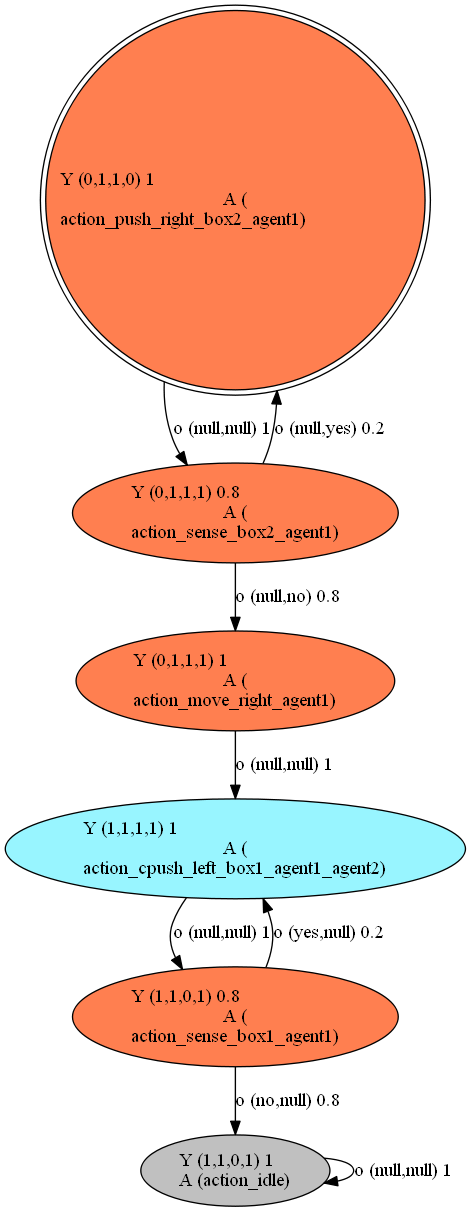
\includegraphics[width=0.25\textwidth,height=\textheight,keepaspectratio]{Agent1-Graph.dot.png}}
%       \hfill
%     \subfloat[After]{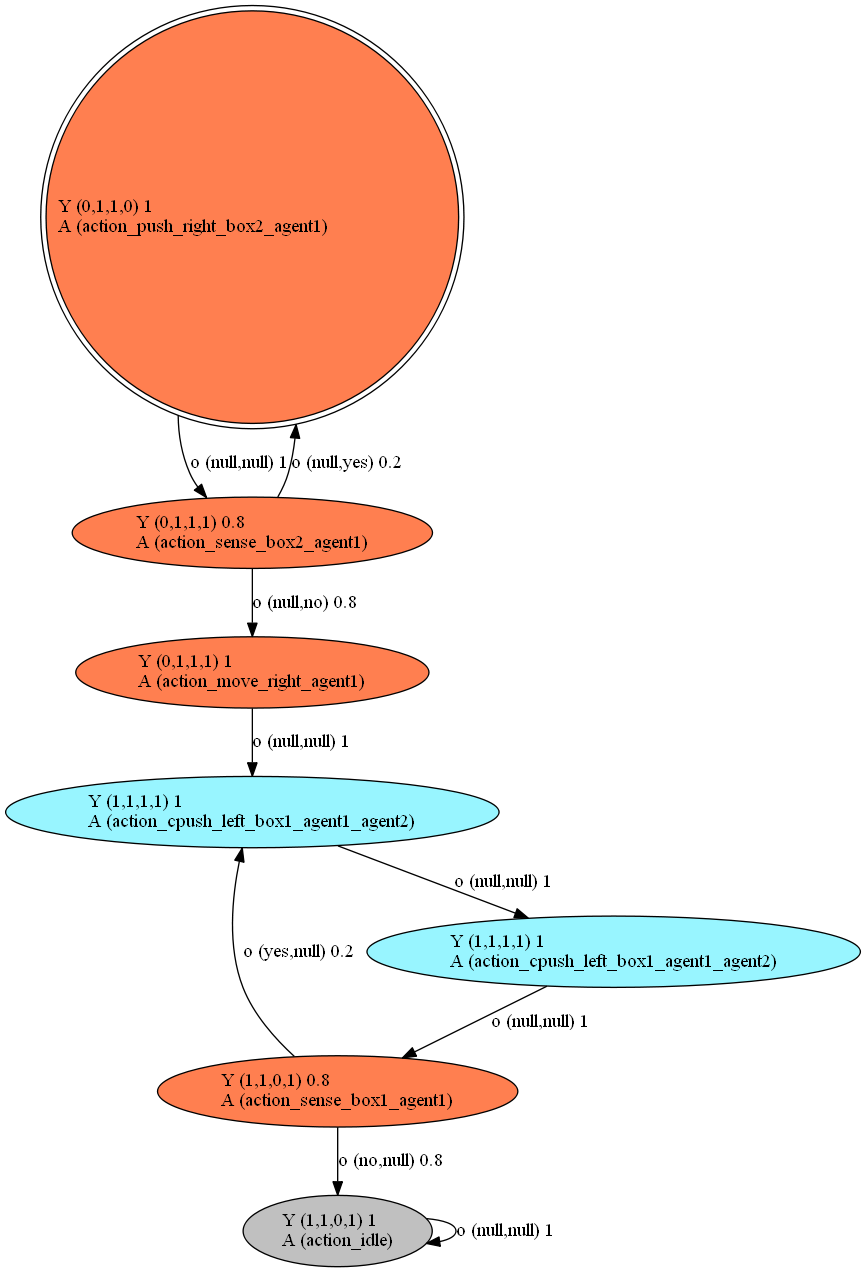
\includegraphics[width=0.4\textwidth,height=\textheight,keepaspectratio]{Agent1-Graph-Aligned.png}}
% \caption{\label{Fig:Alignment} \emph{Agent1}'s Policy}
% \end{figure}
% \end{example}

\begin{figure}
    \centering
    \subfloat{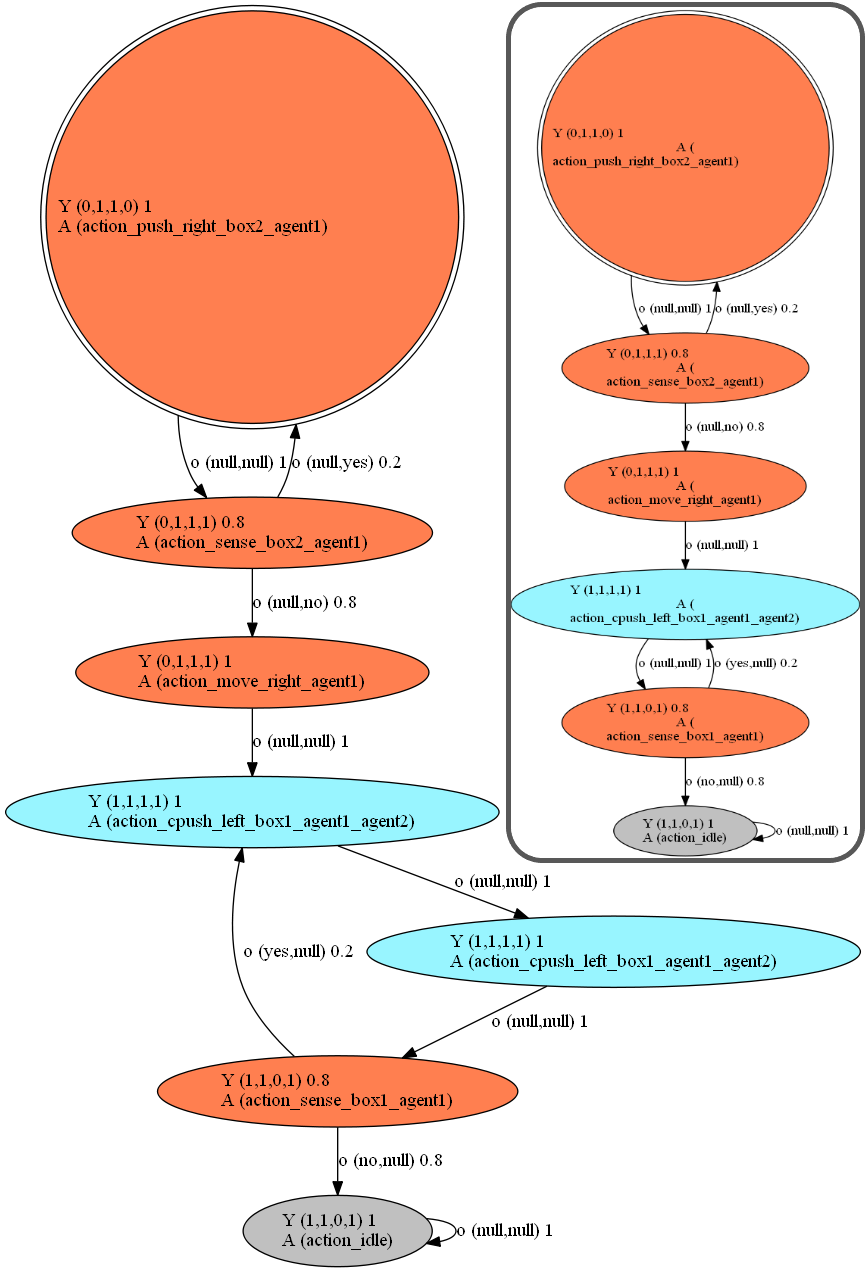
\includegraphics[width=0.39\textwidth,height=\textheight,keepaspectratio]{Agent1-Both-Graphs.png}}
\caption{\label{Fig:Alignment} \emph{Agent1}'s Policy, Before (framed) And After Alignment and Adjustments.}
\end{figure}
\end{example}

\commentout{
\begin{algorithm}
\caption{Alignment Iteration}
\begin{algorithmic}[tbph]
\State Input: PolicyGraphs $G_1, \ldots, G_M$
\For{$G_i,  i\in\{1, \ldots, M\}$}
	\State {$\mathit{NoopsReqs} \gets \mathit{VertexToIntMapping}$}
      \State {$\mathit{CurrBFS} \gets \Call{BFS}{G_i}$}
      \While {$\mathit{CurrBFS.queue}$ is not empty}
	\State {$v \gets \mathit{CurrBFS.queue.pop}$}
	\State {$a \gets v.action$}
	\If {$a$ is public action}
	\State {$\mathit{identifier} \gets \Call{GetIdentifier}{v}$}
	\State {$\mathit{MaxNoop} \gets 0$}
	\For {$G_j,  j\in\{1, \ldots, M\}\setminus\{i\}$}
	\State {$\mathit{CurrNoop} \gets \Call{NoopReq}{G_j, \mathit{identifier}}$}
	\State {$\mathit{MaxNoop} \gets max(\mathit{MaxNoop}, \mathit{CurrNoop})$}
	\EndFor
	\State {$\mathit{NoopsReqs}[v] \gets \mathit{MaxNoop} - \mathit{CompensationTerm}$}
	\EndIf
	\EndWhile
	\State {$G_i' \gets \Call{AddNoops}{G_i, \mathit{NoopsReqs}}$}
\EndFor
\State {return $G_1', \ldots, G_M'$}
\end{algorithmic}
\end{algorithm}
}

\section{Empirical Evaluation}

We provide experimental results for three domains.
The experiments were conducted on variations of the popular cooperative box pushing, decentralized tiger and rock sampling problems.
We compare our algorithm, FDMAP, with two Dec-POMDP solvers, GMAA-ICE \cite{GMAAICE} and JESP \cite{JESP}, using MADP-tools. \cite{MADP}.
We evaluate FDMAP, GMMA-ICE and JESP on a Linux machine with 2 cores and 8GB of memory. (e2-standard-2 type in Google Cloud Platform)

\subsection{\cbp}

In the cooperative box pushing domain, agents on a grid can move and push boxes in four principle directions,
or perform a {\em no-op}. Light boxes can be pushed by a single agent, while heavy boxes can only be pushed by a collaborative push of two agents. 
All actions except for the push actions are deterministic.

Each grid cell can contain any number of agents and boxes, and each agent can sense for a box at its present location.
Initially, each box can appear in either the target cell (and hence, need not be moved) or the lower right cell, with equal probability.
The goal of the agents is to move the boxes to a target cell, located at the upper left corner of the grid.
Action costs are: 10 for {\em Move}, 1
for sensing actions, 30 for {\em Push}, 20 (per agent) 
for {\em Collaborative Push} and 0 for {\em no-op}. The reward for moving a box to its target position is 500. In addition, there's a penalty of 10000 for pushing a box \emph{out} of the target cell to avoid abuse. In configurations with heavy boxes we double the reward and penalty.
% A domain instance of $m$ cells with $n$ agents, $l$ light boxes, and $h$ heavy boxes, has $m^{n+l+h}$ states, $(5\cdot(l+1)+4h\cdot(n-1))^n$ actions and $3^n$ observations.

% Evidently, the box pushing domain calls for longer horizon policies, rather than good local reactive policies, and requires careful coordination to ensure that collaborative push actions are performed simultaneously by the agents.

\subsection{\cdt}
We adapt the Dec-Tiger problem presented in \cite{JESP}. Each agent has a location state variable, which it can alter using a deterministic move action. The tiger also has a location state variable, which resets following a door opening. We differentiate between collaborative and regular opening actions. Finally, we allow the agents to independently receive informative observations, as we don't handle collaborative sensing actions. The reward function is essentially the same - the agent pays 1 for listening, 100 for opening the tiger door alone, and 25 for collaboratively opening the tiger door (0 for move and idle actions). It receives a reward of 10 for either opening the prize door alone or collaboratively. The domains favors collaboration in terms of the penalty.

\subsection{\drs}
In this domain, two rovers start in a grid which is divided into control areas, one per rover, where rocks are spread and needed to be sampled. The rovers can move around the grid, sense the rocks' quality, and sample them. Each rock can be either good or bad for sampling depending on its condition, which is unknown to the rovers. Agents are rewarded for sampling all the good rocks in their control area, but penalized directly for sampling a bad quality rock. Once a good quality rock is sampled, it turns bad. The areas controlled by the rovers
have a non-empty overlap in which both rovers can act.
The rovers are equipped with a long range sensor, whose quality deteriorates according to the range from which it samples a rock. Its maximal sensing ability has 10\% error rate.
The costs are 1 and 5 for sense and move actions, while the penalty for sampling a bad rock is 500, and the reward for sampling all good rocks in a control area is 750.


\begin{figure}
    \centering
    \subfloat{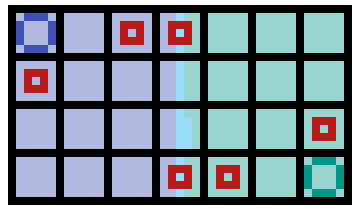
\includegraphics[width=0.3\textwidth,height=\textheight,keepaspectratio]{drsgrid.png}}
\caption{\label{Fig:DRS} \drs. The agents are located in the grid's corners, and their corresponding control area is colored similarly, and the rocks are the red squares, whose condition is unknown. The middle column is the shared zone.}
\end{figure}



\subsection{Settings} 

GMAA-ICE and DP-JESP require an horizon specification, while FDMAP computes a policy for an unbounded horizon. Therefore, we specify the maximal reached planning horizon for them under the column -H-, and for FDMAP we specify the average number of steps until reaching the goal state, under the column -Avg-. In some cases, instead of -Avg-, we specify the -H- column for FDMAP as well, which stands for the simulation length. Discount factor is set to $\gamma=0.99$.
%
For GMAA-ICE and DP-JESP we report the computed policy value. For FDMAP we measured the average discounted accumulated reward of 1000 simulations.
%
We provide results on several configurations of \cbp, \drs , and the known configuration of \cdt.

In \cbp, each box starts at either the top-left or bottom-lower corner with equal probabilities. The problem name is composed of 5 elements specified in brackets, $\textit{BP}-[w][h][n][l][h]$. These
elements denote
Width, Height, Number of agents, Number of light boxes, ans Number of heavy boxes.
% For 1 dimensional grids, DP-JESP and GMAA-ICE were given a minimalistic version of the problem that does not include unnecessary actions | push and move for the up and down directions | to decrease the domain size.
We specify the agents' initial locations (denoted by $I$), as well as the domain size ($S$ and $A$), alongside the configuration name.

In \cdt, each agent starts in a known location, while the tiger location is unknown, and has equal probability for each side.

In \drs, the agents start at the bottom right and upper left corners, and the rocks at known locations depending on the grid size. We experiment with different grid widths and rocks amounts, specified in the domain name with two corresponding marks, $\textit{DRS-[w][r]}$.

All planners were given a total of 1 hour  to solve each $\langle\textit{configuration, horizon}\rangle$ pair. We report running times in seconds. The time shown for DP-JESP and GMAA-ICE is based only on its log from MADP-Toolbox, and does not include the problem loading, which is in many cases non negligible. FDMAP time does not include writing the SARSOP policies and graphs to disk, as they are highly dependent on hardware quality and can effectively remain in memory throughout the whole process - this can be solved using RAM drive or RAM file system abstractions.

% In both GMAA-ICE and DP-JESP, configurations BP-32302, BP-32303 and BP-33221 could not be solved for any horizon. Therefore we provide comparisons only for the first four configurations (Table \ref{tbl:scale}), while the harder configurations are shown in Table \ref{tbl:maxres}. We also provide a more sensitive analysis of the horizon in table \ref{tbl:small}

%In DP-JESP, $\times$ marks a timeout. In GMAA-ICE we mark two different timeout options: FF refers to failure of finding a full policy for the required horizon, where FH refers to an earlier stage timeout when computing the heuristic function.
%\eliran{I want to remove the above paragraph since FH occurred only in the largest configurations, which I now centralized in a single table that doesn't even report the competing solvers' results. Is it ok? (FH is the more severe timeout, so it just acts in their favor).}


\subsection{Results}

\begin{table}
\centering
\scriptsize
    \resizebox{\columnwidth}{!}{
    \vspace{-20em}
    \begin{tabular}{|c||c||c||c||c||c|}
         \hline
         \multicolumn{6}{|c|}{FDMAP}\\ 
         \hline
         Problem & MaxSteps & AvgSteps & Time & Value & \%Wins\\
         \hline
         BP-32302 & & & & & \\
         $|S|=7776, |A|=3375$ & 31 & 12 & 89.83 & 275.76 & 100 \\
         $I=\langle(1,2),(1,3),(2,3)\rangle$ & & & & & \\
         \hline
         BP-32303 &&&&& \\
         $|S|=46656, |A|=8000$ & 45 & 18 & 2210.28 & 406.22 & 100 \\
         $I=\langle(1,2),(1,3),(2,3)\rangle$ & & & & & \\
         \hline
         BP-33221 &&&&& \\
         $|S|=59049, |A|=324$ & 110 & 43 & 2863.08 & 125.23 & 99 \\
         $I=\langle(1,3),(3,1)\rangle$ & & & & & \\
         \hline
         BP-33221 &&&&& \\
         1800 seconds per agent & 121 & 39 & 3014.04 & 321.81 & 100 \\
         &&&&&\\
         \hline
         DRS-5424 &&&&& \\
         $|S|=9216, |A|=143$ & 33 & 21 & 2537.10 & 1121.12 & 97\\
         &&&&&\\
         \hline
         DRS-7424 &&&&& \\
         $|S|=16384, |A|=143$ & 38 & 23 & 3310.95 & 1045.74 & 97 \\
         &&&&&\\
         \hline
    \end{tabular}}
    \caption{\label{tbl:maxres} Results for the largest scale problems, which only FDMAP managed to solve. Running times are rapidly increasing while reaching the scales limit of the underlying POMDP solver. The policies are still very robust, and reach the goal state in most cases (\%Wins). MaxSteps and AvgSteps specify the maximal and average number of steps made until reaching a goal state throughout the runs.}
    
\end{table}

\begin{table}
\centering
\scriptsize
    \resizebox{\columnwidth}{!}{
    \begin{tabular}{|c|c|c||c|c|c||c|c|c|}
         \hline
         \multicolumn{3}{|c||}{DP-JESP} & \multicolumn{3}{c||}{GMAA-ICE} & \multicolumn{3}{c|}{FDMAP}\\
         \hline
         \multicolumn{9}{|c|}{BP-31211 $|S|=81, |A|=16, I=\langle(1,2),(1,3)\rangle$} \\
         \hline
         H & Time & Value & H & Time & Value & Avg & Time & Value \\
         \hline
         4 & 1861.30 & 279 & 4 & 30.23 & 330.07 & 15 & \textbf{6.07} & \textbf{613.98} \\
         \hline
         \hline
         \multicolumn{9}{|c|}{BP-22202 $|S|=256, |A|=225,
         I=\langle(1,2),(2,2)\rangle$} \\
         \hline
         H & Time & Value & H & Time & Value & Avg & Time & Value \\
         \hline
         3 & 267.24 & 271 & 3 & 160.18 & 320.46 & 9 & \textbf{7.08} & \textbf{348.56} \\
         \hline
         \hline
         \multicolumn{9}{|c|}{BP-22203 $|S|=1024, |A|=400,
         I=\langle(1,2),(2,2)\rangle$} \\
         \hline
         H & Time & Value & H & Time & Value & Avg & Time & Value \\
         \hline
         2 & \textbf{59.06} & 0 & 2 & 1053.27 & 414 & 17 & 125.50 & \textbf{514.09} \\
         \hline
                  \hline
         \multicolumn{9}{|c|}{DRS-3421 $|S|=512, |A|=90$} \\
         \hline
         H & Time & Value & H & Time & Value & Avg & Time & Value \\
         \hline
         3 & 314.35 & 224.38 & 3 & \textbf{82.86} & 738.88 & 18 & 1725.80 & \textbf{1027.88} \\
         \hline
         \hline
         \multicolumn{9}{|c|}{DRS-3422 $|S|=1024, |A|=100$} \\
         \hline
         H & Time & Value & H & Time & Value & Avg & Time & Value \\
         \hline
         3 & \textbf{1081.41} & 518.19 & 3 & 2867.06 & 507.76 & 20 & 2438.82 & \textbf{1048.11} \\
         \hline
         \hline
         \multicolumn{9}{|c|}{DRS-5422 $|S|=2304, |A|=100$} \\
         \hline
         H & Time & Value & H & Time & Value & Avg & Time & Value \\
         \hline
         3 & \textbf{1838.84} & 111.25 & 3 & $\times$ & - & 16 & 2434.88 & \textbf{1157.95} \\
         \hline
    \end{tabular}
    }
    \caption{\label{tbl:scale}
    FDMAP outperforms DP-JESP and GMAA-ICE with respect to policy value in both domains, and also with respect to running time in Box-Pushing. Results for DP-JESP and GMAA-ICE are for maximal horizon reached, specified under the -H- column. In FDMAP we present the average number of steps until reaching the goal state when running the policy for an unbounded number of steps, specified under the -Avg- column.}
    \vspace{0.5cm}
    {
    \begin{tabular}{|c||c|c||c|c||c|c|}
         \hline
         \multicolumn{7}{|c|}{\cdt,  $|S|=8, |A|=5, I=\langle(0,1,0),(0,1,1)\rangle$} \\
         \hline
         H & \multicolumn{2}{|c||}{DP-JESP} & \multicolumn{2}{c||}{GMAA-ICE} & \multicolumn{2}{c|}{FDMAP}\\ 
         \hline
         & Time & Value & Time & Value & Time & Value \\
         \hline
         3 & 0.42 & 1.96 & \textbf{0.24} & \textbf{11.15} & 6.63 & 11.10 \\
         \hline
         4 & 33.15 & 10.05 & 841.67 & \textbf{11.03} & \textbf{"} & 9.12 \\ 
         \hline
         5 & 1792.22 & 5.78 & $\times$ & - & \textbf{"} & \textbf{8.56} \\
         \hline
         6 & $\times$ & - & $\times$ & - & " & 9.05 \\
         \hline
          10 & $\times$ & - & $\times$ & - & " & 10.19 \\
         \hline
          20 & $\times$ & - & $\times$ & - & " & 16.42 \\
         \hline
          30 & $\times$ & - & $\times$ & - & " & 20.10 \\
         \hline
          40 & $\times$ & - & $\times$ & - & " & 24.62 \\
         \hline
         Max & 33.15 & 10.05 (4) & \textbf{0.24} & 11.15 (3) & 6.63 & \textbf{29.25} (49) \\
         \hline
    \end{tabular}
    }
    \caption{\label{tbl:dt} Results for \cdt. FDMAP manages to obtain competitive results on small horizons, while demonstrating a consistent value improvement in larger horizons.}

\end{table}

\begin{table}
\centering
\scriptsize
    \resizebox{\columnwidth}{!}{
    % Our policy graph's longest Hamiltonian path is of length 12 - this implies that a maintainable coordination was found, which does not break after a single cycle.}
        \begin{tabular}{|c|c|c||c|c|c||c|c|c|}
         \hline
         \multicolumn{3}{|c||}{DP-JESP} & \multicolumn{3}{c||}{GMAA-ICE} & \multicolumn{3}{c|}{FDMAP}\\
         \hline
         \multicolumn{9}{|c|}{BPPEN-31211 $|S|=81, |A|=16, I=\langle(1,2),(1,3)\rangle$} \\
         \hline
         H & Time & Value & H & Time & Value & Avg & Time & Value \\
         \hline
         3 & 25.95 & 0 & 4 & 79.28 & 265.44 & 15 & \textbf{8.54} & \textbf{586.96} \\
         \hline
         \hline
         \multicolumn{9}{|c|}{BPPEN-22202 $|S|=256, |A|=225,
         I=\langle(1,2),(2,2)\rangle$} \\
         \hline
         H & Time & Value & H & Time & Value & Avg & Time & Value \\
         \hline
         3 & 495.61 & 135.40 & 3 & 446.03 & 213.79 & 9 & \textbf{11.66} & \textbf{354.29} \\
         \hline
         \hline
         \multicolumn{9}{|c|}{BPPEN-22203 $|S|=1024, |A|=400,
         I=\langle(1,2),(2,2)\rangle$} \\
         \hline
         H & Time & Value & H & Time & Value & Avg & Time & Value \\
         \hline
         2 & 38.70 & 0 & 2 & 1054.5 & 326.50 & 15 & \textbf{31.09} & \textbf{510.13} \\
         \hline
    \end{tabular}}
    \caption{\label{tbl:bppen}Results for a variation of \cbp, in which we penalize an agent for pushing a light box blindly.}
\end{table}

\begin{table}
\centering
\scriptsize
    \resizebox{\columnwidth}{!}{
    \begin{tabular}{|c||c|c||c|c||c|c|}
         \hline
         \multicolumn{7}{|c|}{BP-21210 $|S|=8, |A|=16, I=\langle(1,1),(1,2)\rangle$} \\
         \hline
         H & \multicolumn{2}{|c||}{DP-JESP} & \multicolumn{2}{c||}{GMAA-ICE} & \multicolumn{2}{c|}{FDMAP}\\ 
         \hline
         & Time & Value & Time & Value & Time & Value \\
         \hline
         4 & 19.87 & 0 & \textbf{1.15} & \textbf{426.91} & 3.40 & 306.62 \\
         \hline
         5 & 1069.95 & 0 & 2.09 & 438.34 & " & 301.56 \\ 
         \hline
         6 & $\times$ & - & 6.97 & 448.19 & " & 357.44 \\
         \hline
         7 & $\times$ & - & 8.98 & 450.97 & " & 412.54 \\
         \hline
         Max & 1069.95 & 0 (5) & 17.1 & \textbf{454.70} (25) & \textbf{3.40} & 412.54 (7) \\
         \hline
    \end{tabular}
    }
    \caption{\label{tbl:small} FDMAP outputs a reasonable value compared to GMAA-ICE, which optimizes the small scaled problem. The last row presents results for the maximal horizon reached on DP-JESP and GMAA-ICE, and average simulations steps until reaching the goal state for FDMAP when run for unbounded number of steps. These are specified in parentheses next to the policy value.}
\end{table}

Results are presented in Tables \ref{tbl:scale}, \ref{tbl:dt}. These problems call for
solutions of different types.
\cdt\ rewards or penalizes the agent for any single move, requiring local and reactive planners.
Next comes \cbp, which rewards the agents for pushing a box to the target tile, aggregating a chain of well-directed pushes of a box to a single reward.
Finally, \drs\ rewards an agent only for achieving all of its objectives, which makes large-horizon planning ability crucial, giving no reward at all to partial solution.
%\ronen{don't understand the above. seems like you are repeating the properties of the domains}\eliran{I see we only stated it previously in the end of 4.1. I think this would be a good place to present them, since our conclusions are drawn based on these properties. Should we remove it from 4.1?}
%\ronen{yes. no point of repeating in the same section}\eliran{I removed it from 4.1 then, it appears only here now.}

We can see that FDMAP manages to produce policies with higher quality when considering large horizons. We also see that FDMAP's planning time is
significantly lower in \cbp\ and \cdt\ compared to GMAA-ICE and JESP.  This is due to the fact that FDMAP does not plan directly on the decentralized model, but rather solves multiple POMDP models, which are known to require much less computational effort~\cite{DECPOMDPCOMP}.

In addition, the running time of FDMAP is significantly higher in \drs\ compared to configurations of similar scale in \cbp. The underlying POMDP solver is extremely affected by the number of uncertain components in the world, which is higher in \drs~(3-6) compared to the other domains, \cbp\ and \cdt~(1-3).

%\ronen{What "manages to reduce"?}\eliran{reformulated, should we elaborate on that? It seems that this number (of uncertain components) affects the running time much more than the sheer number of states. It's of course directly related to the underlying POMDP solver, which takes most of the computation time.}

In Table \ref{tbl:maxres}, FDMAP still manages to produce good quality policies on the largest domains, yet with longer running times. The size of the hardest configuration, BP-33221, approaches the maximal problems that SARSOP \cite{SARSOP} can solve.

Tables \ref{tbl:small} and \ref{tbl:dt} show that FDMAP manages to produce reasonable results compared to the other solvers even when dealing with extremely small configurations and horizons in which optimal solvers such as GMAA-ICE can excel.

To observe the difference between the policies FDMAP produces to the ones GMAA-ICE does, we present another variation of \cbp, where we add a penalty to light boxes push actions that occur with no box in the cell. Table \ref{tbl:bppen} presents the results (configuration name prefixed with BPPEN). We can see that the the reward difference on maximal results compared to Table \ref{tbl:scale} are much lower for FDMAP, indicating that FDMAP's policies in the non-penalized configurations exploit the horizon and favors sensing over blind pushing, leading to higher-quality results.

The need for large horizon planning, which was mentioned in several contexts of reward shaping \cite{REWARDSHAPING,REWARDSHAPING2}, becomes most evident in \drs, where the problem's objective cannot be achieved, even partially, in small horizons.
In these scenarios, scaling to large horizons becomes crucial and leads to significantly higher solution qualities as can be seen in Tables~\ref{tbl:scale} and~\ref{tbl:maxres}.

\section{Summary}
We presented FDMAP --- an algorithm for solving factored Dec-POMDPs. FDMAP begins by solving a centralized POMDP, which we call the team POMDP, obtaining a team plan. Then, FDMAP creates agent specific POMDPs whose solutions encourage agents to complete their role in the team plan. The agent plans are then aligned for synchronization between the agents. We experimented with three domains on various configurations which require collaboration and coordination in both long and short horizons, showing that we can scale to much larger problems and horizons than current Dec-POMDP solvers, while computing good quality policies. 

Our decomposition approach is based on intuitive steps,
and performs well, but the concrete instantiation of the projection to single-agent problems and their alignment includes many heuristic choices. While these choices are driven by sensible intuitions, future work should seek to examine alternatives and use more principled choices for generating the single-agent rewards and aligning the solution. We believe this can be a fruitful ground for future interesting developments.


\commentout{
There are two direction in which we deem FDMAP can be improved, in both scalability and theoretical guarantees.
The use of online planners instead of SARSOP as the underlying POMDP solver, can greatly improve the scale of solvable problems. The changes in terms of algorithm's structure are minor, as we merely need to be able to produce the single agent policy graphs using an online solver.
In terms of theoretical guarantees, a deeper examination of domain properties should be conducted, in order to understand the intricacies of a Factored Dec-POMDP model that allow FDMAP, or prevent it from, providing high quality solutions. A possible direction would be further research of the "anchoring" variables definition that was presented, as a measurement of the amount of uncertainty that resides in the domain, whose effect on the computation time was extremely salient.
Furthermore, a yet untouched region we expect FDMAP to struggle in are domains in which the optimal \emph{team} solution does not coincides with the decentralized one, a phenomena that would turn the reward shaping process to obsolete, and would require careful adaptations, involving an interaction with both the team and the decentralized problems, in order to properly shape the rewards.

% In terms of solution quality, we aim at using more principled methods of reward shaping, that come from the field of reinforcement learning in forms of multi-objectivization \cite{REWARDSHAPING}.
% Our goal would be to convert the concept of contexted actions into objectives of each agent, while preserving optimality with respect to the decentralized problem. In addition to improving quality already solvable domains, it can help better tackle the problems of reward-cycles \cite{RLCYCLES} or the need for anchor variables, and enlarge our scope of solvable problems.

\section*{Acknowledgements}
This work was supported by ISF Grant 1651/19, by the Israel Ministry of Science and Technology Grant 54178, and by the Lynn and William Frankel Center for Computer Science.
}

%\fontsize{9.6}{10.6}\selectfont
\bibliography{bibilography.bib}
\end{document}